%----------------------------------------------------------------------------------------
%	PACKAGES AND OTHER DOCUMENT CONFIGURATIONS
%----------------------------------------------------------------------------------------

\documentclass[paper=a4, fontsize=11pt]{scrartcl} % A4 paper and 11pt font size
\usepackage[bottom=1.2in]{geometry}

\usepackage[T1]{fontenc} % Use 8-bit encoding that has 256 glyphs
\usepackage{fourier} % Use the Adobe Utopia font for the document - comment this line to return to the LaTeX default
\usepackage[english]{babel} % English language/hyphenation
\usepackage{amsmath,amsfonts,amsthm} % Math packages

\usepackage{sectsty} % Allows customizing section commands
\allsectionsfont{ \rmfamily\scshape} % Make all sections centered, the default font and small caps

\usepackage{fancyhdr} % Custom headers and footers
\pagestyle{fancyplain} % Makes all pages in the document conform to the custom headers and footers
\fancyhead{} % No page header - if you want one, create it in the same way as the footers below
\fancyfoot[L]{} % Empty left footer
\fancyfoot[C]{} % Empty center footer
\fancyfoot[R]{\thepage} % Page numbering for right footer
\renewcommand{\headrulewidth}{0pt} % Remove header underlines
\renewcommand{\footrulewidth}{0pt} % Remove footer underlines
\setlength{\headheight}{13.6pt} % Customize the height of the header

\numberwithin{equation}{section} % Number equations within sections (i.e. 1.1, 1.2, 2.1, 2.2 instead of 1, 2, 3, 4)
\numberwithin{figure}{section} % Number figures within sections (i.e. 1.1, 1.2, 2.1, 2.2 instead of 1, 2, 3, 4)
\numberwithin{table}{section} % Number tables within sections (i.e. 1.1, 1.2, 2.1, 2.2 instead of 1, 2, 3, 4)

\setlength\parindent{0pt} % Removes all indentation from paragraphs - comment this line for an assignment with lots of text

\usepackage[margin=2cm]{caption}
\usepackage{listings}
\usepackage{subcaption}
\usepackage{graphicx}
\newcommand{\aat}{\textbf{AAT}}
\newcommand{\hit}{\textbf{Hit Time}}
%----------------------------------------------------------------------------------------
%	TITLE SECTION
%----------------------------------------------------------------------------------------

\newcommand{\horrule}[1]{\rule{\linewidth}{#1}} % Create horizontal rule command with 1 argument of height

\title{	
\normalfont \normalsize 
\textsc{Georgia Institute of Technology } \\ [25pt] % Your university, school and/or department name(s)
\horrule{0.5pt} \\[0.4cm] % Thin top horizontal rule
\huge RPC-Based Proxy Server \\ % The assignment title
\horrule{2pt} \\[0.5cm] % Thick bottom horizontal rule
}

\author{Group member : \\
\\
 Xiong Ding 902934749 \\ 
 Yuebin Zhou 903005133
} % Your name

\date{\normalsize\today} % Today's date or a custom date

\begin{document}

\maketitle % Print the title

%----------------------------------------------------------------------------------------
%	part 1
%----------------------------------------------------------------------------------------

\section{Introduction}

In this project, we build a Remote Procedure Call based proxy server. Remote procedure call is an IPC that could enable a program to execute on another computer through network. This could be used to build a client-server model. Proxy server is a model that the server is acting like the proxy of clients. It will take the URLs sent by clients and then go to fetch those pages. While getting those pages, the server will simultaneously send back them to clients. 

\vspace{1em}

In server client model, caching is a necessary part. It could help to increase the page loading performance as well as decrease the transmit load. There are all kinds of caching policies which caters for different use patterns. In this project, we build three different caches: 
\textbf{Random} Cache, \textbf{First-In-First-Out} Cache(FIFO) and
\textbf{Least Recently Used} Cache(LRU). We measured these three caches plus \textbf{No Cache} with respect to hit rate and elapsed time. The experiment shows different performances of different caching policies. Advantages and disadvantages of different caching policies are reflected in our experiments.

\vspace{0.5em}

To ease the development of this project, we utilized two software libraries. \textbf{Apache Thrift} was leveraged to build the RPC based server. Apache Thrift is a software that could generate code framework to build cross-language services. 
\textbf{Libcurl} is another one that we used. It is a powerful library for server communication. It supports HTTP GET/PUT/POST functions. Proxy server would use them to fetch and send pages. Client would use them to send URLs and receive document bodies of web pages. 



\section{Cache Design}

Cache is implemented by the combination of \textbf{Hash table} 
and \textbf{doubly linked list}. Each hash entry is 
a tuple \textbf{<URL, node*>}, where the node pointer points to a node
in the doubly linked list (cache list). Each node is a structure
containing the URL and the corresponding web page content.

\vspace{0.5em}

We use the C++ STL container \textbf{std::unordered\_map} to hold the 
hash table. The searching operation in the unordered\_map
has an average complexity of $O(1)$, and the worst case is $O(N)$. Doubly
linked list is used to hold the cached web pages. We insert new nodes
to the head, and remove nodes from the tail. Different cache policies will
implement different rules to manipulate this list, and insertion and
deletion operations has complexity $O(1)$.

\vspace{0.5em}

The cache class can support two different operations: \textbf{get()} and
\textbf{put()}. whenever there comes a URL, \textbf{get()} will try to look
up the hash table, if the corresponding entry is found, then the web page
content would be returned. 
\textbf{get()} may also modify the node list to reflect recent access
(only for LRU policy). On the other hand, \textbf{put()} function is
responsible for inserting new node to list and deleting nodes if the
total size of cache goes beyond the limit. Therefore, different cache 
policies only need to implement different \textbf{get()} and 
\textbf{put()}, 
such that the interface keeps uniform.

\section{Cache Policies}

\subsection{LRU}
The Least Recent Used policy will keep track of the access order 
of cache list. In our implementation, the closer to the list head, 
the fresher of the web page contained in this node. So every time 
there is a cache hit, the corresponding cache node will be moved to
the head. If the cache is full, the nodes closest to the tail will
be removed first.
\begin{itemize}
\item \textbf{Pros:} LRU can enhance locality. Recently visited websites
are likely to be visited again.
\item \textbf{Cons:} Performance issue: every lookup of the cache needs
to update the double linked cache list no matter it is a hit or
miss.
\end{itemize}

\subsection{Random}
Random policy evicts the cache entry randomly When the total cache 
size exceeds the maximal size. It can be implemented by a random
number generator to choose the replace cache entry.
\begin{itemize}
\item \textbf{Pros:} It will not result in extremely bad performance
for some special 
 patterns. Since the eviction decision is not based on the 
access pattern; thus, it has similar performance for all kinds of patterns.
\item \textbf{Cons:} It has higher miss rate compared with other cache 
policies which take account of access pattern like LRU, because users
are likely to browse a few web pages repeatedly.
\end{itemize}

\subsection{FIFO}
The ``first in first out'' policy will evicts the entry that was put 
into the cache earliest. Cache entries are always inserted at the head
of the cache container, and evicted from the tail of the cache container.
\begin{itemize}
\item \textbf{Pros:} The hypothesis of FIFO is that the oldest entry in the cache is least
likely to be accessed again. FIFO reflects the `age' of each cache entry, 
and evicts the oldest page, so it has relatively better performance compared
to random policy.
\item \textbf{Cons:} In some cases, the oldest cache may be accessed again,
such as browsing a few web pages in a circular manner, which results in
a large 
number of cache misses. 
\end{itemize}

\section{Evaluation Metrics}

In order to measure the performance of different cache policies, we come up with two metrics. The first one is \textbf{hit rate}, which is the percentage of cache hit among all web pages acquires. 
More cache hits mean that fewer web pages are needed to be fetched from original websites. This would lead to a better performance. Therefore, the cache policy achieves the highest hit rate would be the one with the best performance in that case. 

\vspace{1em}

Besides hit rate, \textbf{total time of accessing the list of workload}
on the client side is also recorded. It is easy to see that the less the time, the better the performance. One thing to note is that the time should be compared relatively since the network situation is unstable.
Also, these two metrics are related to each other. A higher hit rate will save the time on fetching and caching the web pages. This could help to decrease the elapsed time. The trend is more significant when the network is not good. 

\section{Workloads Generation}

We used two workloads in this experiment. They both are a list of 110 URLs generated from a list of 20 different website URLs. One is a 
\textbf{random workload}. It is generated randomly from the website list. This is simulating a common scenario which users do not show any obvious patterns in visiting websites. Random cache could also be used as a baseline to evaluate all kinds of caches since it is not biased. Another workload we used is repeated workload which is designed for FIFO and LRU cache. This workload is a repeated iteration of the website list with three websites inserted in this list every two, three and four URLs. This is simulating users continuously visiting those frequently visited page in certain order. For example, a GT student may first use google to find T-square and then visit google doc and google scholar to start to work on the report or homework. This is a fixed workflow that always repeats. While in this process, one may frequently visit some websites. For example, that student might frequently visit google to search or facebook to have some fun while studying. This is the reason we periodically insert some websites into the workload.  
    

\section{Experiment Description}

The experiment is conducted on two laptops of team members. The two computers are both running linux system and connected to GTWIFI network. Server program is running on one computer while the client is running on the other one. The client are fed with the host name of the proxy server so that they can build up a connection via socket. 

There are two workloads and three different caching policies plus the no caching, so there are 8 combinations in total. Cache size is also an important factor worth of exploring. Therefore, for each caching policy we used 256K cache, 512K cache, 1M cache and 2M cache to observe the phenomena. For each combination and certain cache size, we let the client to perform a request according to the workload for 5 times. In each time, we record the time that it takes to proxy the whole worklist and the total hit. We then use the hit number to subtract the previous hit to get the hit of this round. Time is obtained from system time. 

We were expecting the LRU and FIFO could show a slightly better or at least similar performance over random cache on random workload, since there are no patterns in this load. However, we expected the LRU and FIFO could be much better than random in repeated workload, because LRU and FIFO are more likely to keep those frequently or recently visited page cache whereas random cache destroys cache items randomly. 

One thing worth to mention is that we found some websites do not support curl. A web document size whose size is zero would be returned if we request it using curl. This will affect our cache performance evaluation. Our solution is to check the size of obtained pages and refuse to cache it if the size is zero. 

\section{Experimental Results \& Analysis}
\begin{figure}[h]
  \centering
  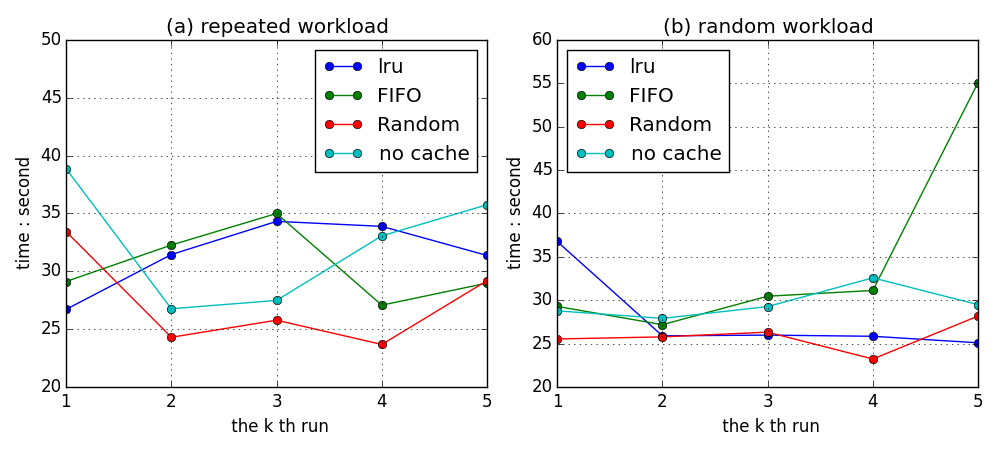
\includegraphics[width=\textwidth]{../data/time256k}
  \caption{cache size = 256k}
  \label{fig:time256k}
\end{figure}
Figure 7.3 shows the elapsed time of different cache policies with a cache size of 256K. As the cache is small, no caching policies are able to show significant performance advantages over no caching. In this case, we could not say any caching policy is doing significantly better than others. The relatively small cache size is the main factor shafting the performance, i.e: no matter how good or bad the caching policies are, good performance cannot be achieved.
\begin{figure}[h]
  \centering
  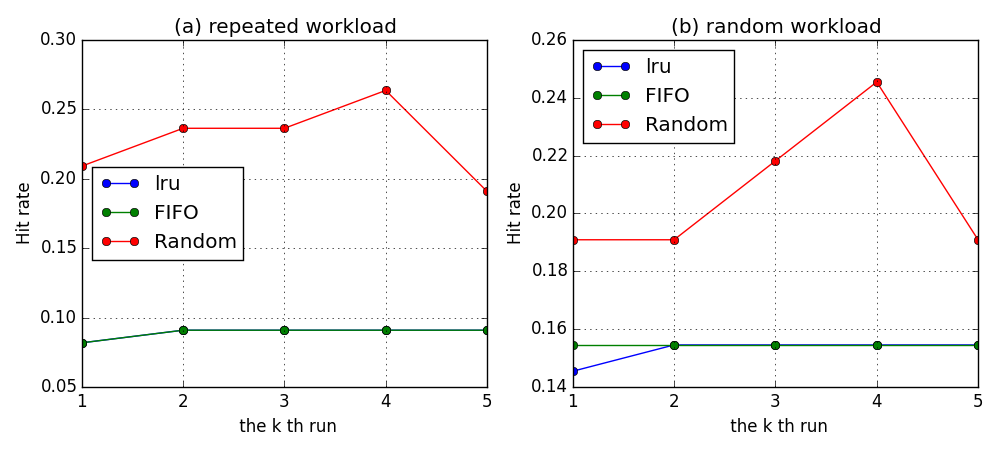
\includegraphics[width=\textwidth]{../data/hit256k}
  \caption{cache size = 256k}
  \label{fig:hit256k}
\end{figure}
Figure 7.4 shows the hit rate of cases where cache size=256k. We were surprised to find the random cache achieves the best performance in this case. Regarding the relatively worse performance of FIFO and LRU in the repeated workload. We think the small cache size is making the cache not able to cache enough number of pages to cover an entire repeating sequence of URLs. So when a repeated URL appear, it would have been removed from the cache, whereas it has a better chance to still live in the random cache. For the random cache. We are thinking that if the cache size is small and the cache is intending to remove less recently or frequently appeared URLs, then 'wrong' URLs would be more likely to be removed considering the workload does not contain many frequently or recently appeared URLs. Our conclusion is that random cache policy should be used when the cache size is limited.    

\begin{figure}[h]
  \centering
  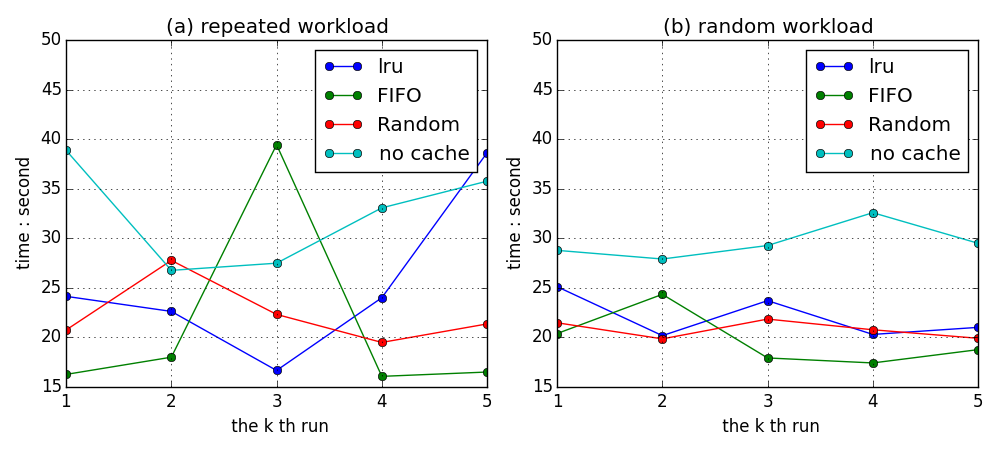
\includegraphics[width=\textwidth]{../data/time512k}
  \caption{cache size = 512k}
  \label{fig:time512k}
\end{figure}
Figure 7.1 shows the elapsed time of visiting two workloads with a cache size of 512K. We can see it takes longer time using no caching under both workloads. This matches our expectation. The other two caching policies are performing likewisely. But LRU does show noticeably shorter time on repeated workload as we expected. Random cache were not doing bad in this case. We think this is because the cache size is just ample, so enough pages might have been cached to keep a good performance no matter what the caching policy is. 
\begin{figure}[h]
  \centering
  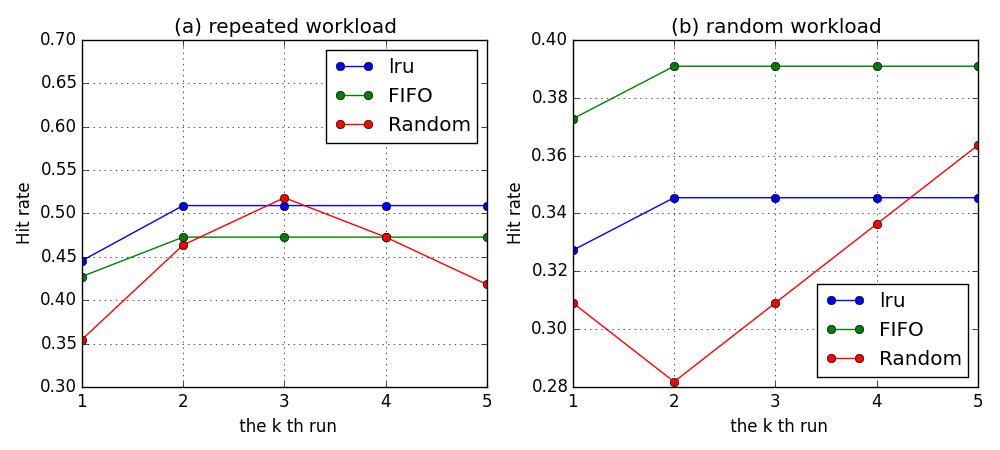
\includegraphics[width=\textwidth]{../data/hit512k}
  \caption{cache size = 512k}
  \label{fig:hit512k}
\end{figure}
The figure 7.2 is showing hit rate in the same scenario which the cache size is 512K. The varying trend of hit rate matches with that of time, which was lower hit rate would lead to longer time and vice versa. Besides this, there are 3 more interest points here. The first one is although running time of random cache is not that slow, the hit rate of random load is significantly lower than the other two. This is what we were expecting. The second one is LRU achieves the highest hit rate in repeated workload. Since this workload is highly repeated, our experiment verified that the LRU would do better in workloads with many repeated URLs. The last point is that FIFO was doing very good. FIFO is suppose to do good in those cases which new URLs are keeping appearing while old URLs are less likely to appear again. We inspected the random workload and found there are several quite long subsequences in that pattern.

\begin{figure}[h]
  \centering
  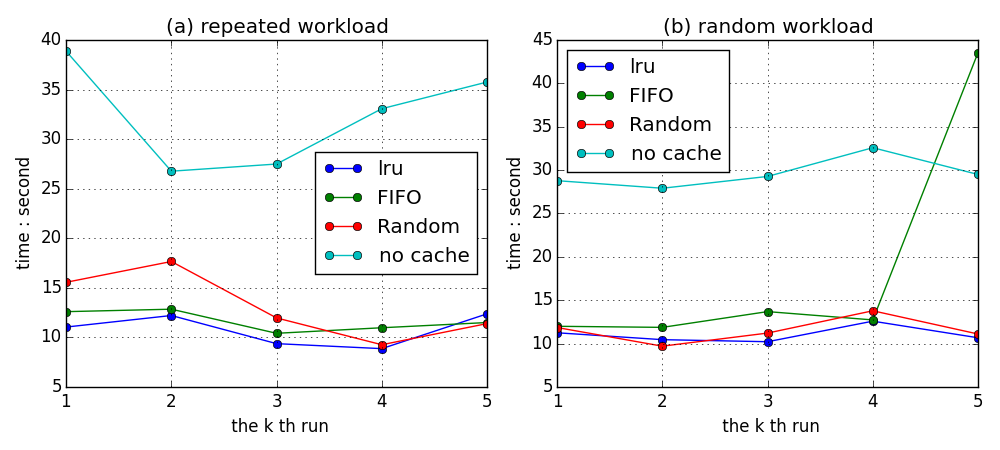
\includegraphics[width=\textwidth]{../data/time1M}
  \caption{cache size = 1M}
  \label{fig:time1M}
\end{figure}
Figure 7.5 shows the time of cases where cache size =1M. Again, cases with no cache are slower than those with caches. We think the advantage of server with cache over that with no cache will be becoming more and more significant along with the augmenting of cache size. In terms of the three caching policies, their running time are converging after we ran them for several rounds. We are guessing this is because 1M size is big enough to full play the power of all kinds of caching policies
\begin{figure}[h]
  \centering
  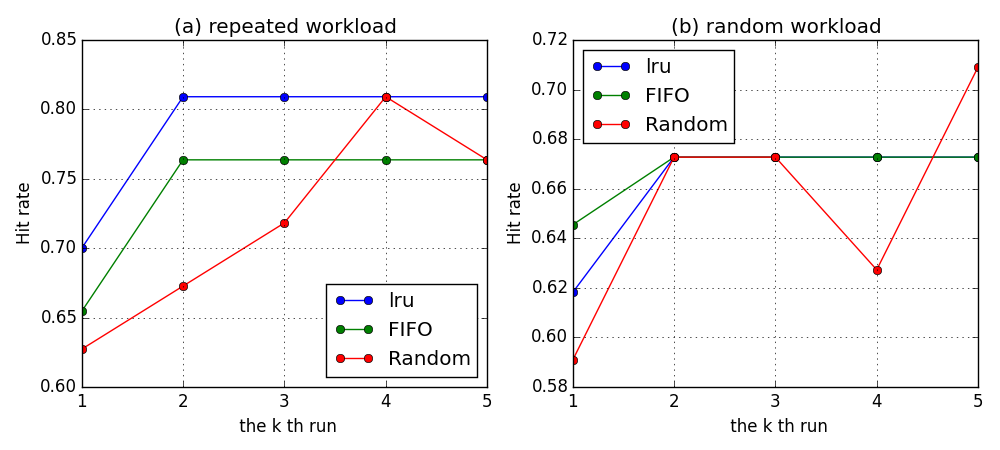
\includegraphics[width=\textwidth]{../data/hit1M}
  \caption{cache size = 1M}
  \label{fig:hit1M}
\end{figure}
Figure 7.6 shows the hit rate in the previous scenarios. The perfect result appears in the repeated load. LRU achieves the best performance while FIFO follows. The random cache is significantly less effective than the other two. This matches our hypothesis very well. We think that cache size is an essential factor in affecting the caching performance. A cache policy could only fully show its power with an appropriate cache size. For random workload, the three cache policy has a similar hit rate. This also matches our expectation. This random workload does not cater for any cache policy, so they neither deteriorate nor improve the hit rate. 
\begin{figure}[h]
  \centering
  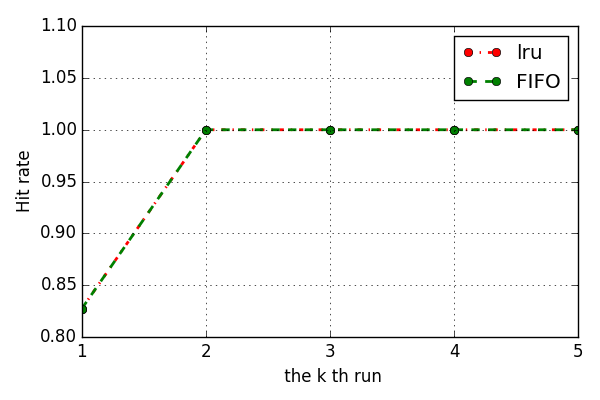
\includegraphics[width=0.7\textwidth]{../data/hit2M}
  \caption{cache size = 2M}
  \label{fig:time2M}
\end{figure}
Finally, we tried 2M cache to reach a saturated situation. We can see from the figure that the hit rate is 1.0 after two rounds. It means the cache has held all pages. From then on, all page transmitted are from the cache. 
\section{Conclusion}
In this project, we successfully built a RPC based proxy server. Besides it, LRU, FIFO and Random cache policy are also implemented. We performed experiments of our implementations on a random workload and a repeated workload to explore and evaluate how different cache policy and cache size can affect the performance of the RPC proxy server. 

From the experiment we draw the following conclusions:
1. As we expected, if the cache size is set to an appropriate value, the performance of cache in a repeated workload is in an order like: LRU>FIFO>Random>No Cache.
2. In random workload with enough cache size, all caches are having a similar performance. They are all significantly better than that of no caching. However, FIFO and LRU may have a worse performance compared to random cache if the cache size is small. 
3. Cache size is an extremely important factor affecting cache performance. An ample cache is necessary for a cache policy to fully play its power. 


\end{document}
